%% LaTeX2e class for student theses
%% sections/content.tex
%%
%% Karlsruhe University of Applied Sciences
%% Faculty of  Computer Science and Business Information Systems
%% Distributed Systems (vsys)
%%
%% Prof. Dr. Christian Zirpins
%% christian.zirpins@hs-karlsruhe.de
%%
%%
%% Version 0.2, 2017-11-15
%%
%% --------------------------------------------------------
%% | Derived from sdqthesis by Erik Burger burger@kit.edu |
%% --------------------------------------------------------

\chapter{
	\iflanguage{english}{Basics for the secure implementation of decentralised social networks}{Grundlagen zur Umsetzung dezentraler sozialer Netzwerke}
}
\label{ch:fundamentals}
\iflanguage{english}{}{
	%Klassen von Anwendungen sowie Implementierungen erläutert.
	Dieses Kapitel gibt einen Überblick über allgemeine Grundlagen von sozialen Netzwerken. Es wird grob erläutert für was soziale Netzwerke gedacht sind; Der Unterschied zwischen zentralen, verteilten, dezentralen und förderierten sozialen Netzwerken herausgestellt sowie auf Sicherheitsaspekte eingegangen.\\
	
	Im Anschluss wird ein Kryptographie Unterkapitel eingeführt in dem die benötigten Verfahren für die sichere Umsetzung erläutert werden. Begonnen wird mit einer kurzen Einführung in Kryptographie. Darauf folgend wird kurz das RSA Verfahren sowie eine allgemeine Beschreibung von Signatur Algorithmen vorgenommen. HTTP Signaturen werden ausführlicher beschrieben, da diese bei der Implementierung des Prototypen verwendet wurden.\\ 
	
	Darauf folgend wird der ActivityPub Standard eingeführt sowie eingeordnet, Bestandteile des Protokolls beschrieben, die Funktionsweise der Client-zu-Server sowie Server-zu-Server Kommunikation und zugehörige Standards kurz erläutert. Des weiteren wird auf die Authentifizierung und Datenintegrität bei ActivityPub eingegangen um damit folgende Fragen zu klären:
	\begin{itemize}
		\item Wie authentifiziert sich ein Benutzer gegenüber dem Server?
		\item Wie stellt man sicher, dass die übertragenen Daten unverändert angekommen sind?
	\end{itemize}
}
\section{
	\iflanguage{english}{General principles of social networks}{Allgemeine Grundlagen sozialer Netzwerke}		
}
	In den Sozialwissenschaften versteht man unter einem sozialen Netzwerk mehrere Personen die miteinander wechselwirkend auf soziale weise interagieren (Vgl. \cite{wikipedia-social-network-sociology}). Die Informatik bildet soziale Netzwerke als Plattformen zum Aufbau und der Pflege von Beziehungen ab. Weiter gefasst können auch Mikroblogging-Dienste, Chat Software, Voice Chat-Programme u. s. w. zu sozialen Netzwerken gezählt werden, da auch die Möglichkeit geboten wird auf soziale Weise miteinander zu interagieren.
	\begin{figure}[h]
		\begin{minipage}{\textwidth}
			\centering
			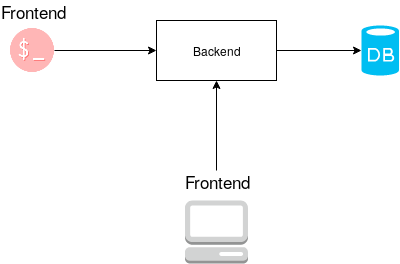
\includegraphics[scale=0.55]{figures/central-social-network.png}
			\label{fig:central-social-network}
			\caption{3 Tier Architektur}
		\end{minipage}
	\end{figure}
	Im Allgemeinen besteht ein soziales Netzwerk aus Softwaretechnischer Sicht aus 3 Komponenten, dies ist aber keine Prämisse. Der Nutzer benutzt das Netzwerk durch eine meist grafische Schnittstelle. Um Zugriff auf dieses zu erlangen benötigt der Nutzer ein \textit{\textbf{Frontend}}. Dies kann in grafischer Form oder als \gls{cli} zur Verfügung stehen. Über das Frontend kann der Nutzer sich nun mit seinen Anmeldeinformationen am \textit{\textbf{Backend}} anmelden und somit meist eine Sitzung eröffnen. Steht ein Web Interface zur Verfügung, werden Sitzungen oft über Clientseitige Cookie Speicherung aufrecht erhalten. Das Backend hat die Aufgabe eingehende Nutzeranfragen entsprechend zu beantworten und, falls autorisiert, die gewünschten Aufgaben auszuführen. Bei größeren sozialen Netzwerken fällt eine große Menge generierter Daten an die verwaltet werden müssen. Dafür wird meistens eine \textit{\textbf{Datenbank}} herangezogen die zumeist auch repliziert betrieben wird. An sich kann ein zentrales Netzwerk auch über den Einsatz von virtuellen Maschinen und Lastenverteilung verteilt oder dezentral sein. Beispielsweise könnte ein zentrales soziales Netzwerk Anfragen länderspezifisch an zuständige Instanzen des Netzwerks weiterleiten. Auch ist es möglich die Daten länderspezifisch zu speichern und somit den Nutzern aus Deutschland andere Inhalte anzubieten als denjenigen aus der Schweiz.\\
	
	\subsection{Verwandte Protokolle}
	Zu Beginn dieses Kapitels wird das Wort Fediverse etwas näher definiert und erläutert worum es sich dabei handelt. Im Anschluss werden mehrere Protokolle die, sowie auch ActivityPub, zum Fediverse gehören vorgestellt.\\
	
	Als erstes soll der Begriff \glqq förderiertes Netzwerk\grqq~von Förderation hergeleitet werden. Unter einer Förderation versteht man den Verbund von etwas. Deutschland ist z. B. ein förderierter Bundesstaat, welcher 16 Bundesländern verbindet. Ein Verbund von Netzwerken wird demnach als Netzwerkverbund, oder auch \glqq förderiertes Netzwerk\grqq, bezeichnet.\\
	
	\glqq Fediverse\grqq~ist ein Kofferwort aus \glqq Federated\grqq~und \glqq Universe\grqq. Historisch gesehen beinhaltete der Begriff nur Microblogging Plattformen die das OStatus Protokoll unterstützen. Mehr zu OStatus \textbf{s. \ref{sub:ostatus}}. Mittlerweile beinhaltet das Fediverse mehr als nur Microblogging Plattformen wie Mastodon\footnote{\url{https://mastodon.social/about}}, sondern auch soziale Netzwerke wie GNU Social\footnote{\url{https://gnu.io/social/}}, sowie \glqq Video hosting\grqq~(PeerTube\footnote{\url{https://joinpeertube.org/en/}}), Plattformen zum veröffentlichen von Inhalten, wie Wordpress, und viele weitere (Vgl. \cite{fediverse}).\\
	
	Im \glqq Fediverse\grqq~dreht sich alles um freie (Open Source) Software anstelle von kommerziellen Produkten. Zudem kann ausgesucht werden welchem Administrator man die Kontrolle über seine Daten geben möchte, anstatt auf eine einzelne Instanz vertrauen zu müssen \cite{fediverse}. Ein weiterer wichtiger Aspekt ist das förderieren von Netzwerken über Protokolle wie OStatus oder Pump.io. Somit kann ein dezentrales soziales Netzwerk durch die Implementierung eines dieser Protokolle zum förderierten sozialen Netzwerk werden.\\
	
	Laut dem Fediverse Netzwerkreport 2018, welcher online zur Verfügung steht, hat sich die Gesamtanzahl der erreichbaren Instanzen von 2.756 auf 4.340 erhöht. Dies entspricht einem Wachstum von 58\%. Die Nutzeranzahl ist von 1.786.036 auf 2.474.601 gestiegen (39\%). Weitere Details sind im Netzwerk Report nachzulesen. Es ist hinzuzufügen das der Netzwerkreport unvollständig ist und Fehler beinhalten kann \cite{fediverse-report}.\\
	
	\subsubsection{OStatus}
	\label{sub:ostatus}
	Der OStatus Standard ist eine Sammlung von verschiedenen nachfolgend gelisteten Protokollen: \textit{Atom, ActivityStreams, WebFinger, WebSub, Salmon, Portable Contacts}\\
	
	Ausgelegt ist der Standard auf das empfangen und versenden von Status Aktualisierungen für förderierte Microblogging Dienste wie Mastodon. Das Zusammenspiel obiger Protokolle ermöglicht den Austausch von Status Aktualisierungen in fast Echtzeit. Profile werden über den WebFinger Standard entdeckt und zusätzlich ist es möglich über das \gls{lrdd} Protokoll die Profile zu entdecken. Um Aktualisierungen zu versenden wird WebSub, unter Zuhilfenahme des ActivityStream Datenformats und Atom, verwendet. Mit Salmon werden Benachrichtigungen versendet\footnote{\url{https://ostatus.github.io/spec/OStatus\%201.0\%20Draft\%202.html}}.
	
	\subsubsection{Diaspora}
	\label{sub:diaspora}
	Diaspora ist ein freier Web Server mit einer integrierten Implementierung eines verteilten sozialen Netzwerkes. In diesem Netzwerk wird ein Knoten als Pod bezeichnet, wobei die Gesamtzahl aller Pod's das Diaspora Netzwerk ausmachen. Durch die integrierte Funktionalität zum sozialen Netzwerken kann auf dem Web Server aufsetzend eine eigene Applikation entwickelt werden.\\ 
	
	Diaspora entdeckt die Profile der Nutzer, wie auch OStatus, über den WebFinger Standard. Zudem wird WebSub verwendet um Echtzeitaktualisierungen zu verteilen. Dies verringert den Verbrauch von Ressourcen auf der Client Seite ausgelöst durch Polling (Vgl. \cite{diaspora-about}). Die Software ist in der Ruby Programmiersprache unter zu Hilfenahme des \glqq Ruby on Rails\grqq~Web Frameworks entwickelt worden. Folgende Modelle sind in dieser Software enthalten (Vgl. \cite{diaspora-introduction}):
	\textit{Benutzer, Personen, Profile, Kontakte, Anfragen, Aspekte, Inhalte, Kommentar, Widerruf}
	
	\subsubsection{Pump.io}
	\label{sub:pumpio}
	Ähnlich dem in dieser Arbeit behandelten Standard werden beim Pump.io Protokoll auch Nutzernachrichteneingänge und Nutzernachrichtenausgänge bereitgestellt. Der Nachrichtenausgang endet hier anstatt auf das Postfix \glqq outbox\grqq, wie bei ActivityPub, auf \glqq feed\grqq. Außerdem nutzen beide das Activity Streams 2.0 Datenformat. Zur Authentisierungen des Clients gegenüber dem Server wird hier das OAuth 1.0 Protokoll verwendet (Vgl. \cite{oauth-1.0-protocol}). Die Nutzerprofile sowie Informationen über den Host werden über die \glqq Web Host Meta\grqq~Spezifikation entdeckt (Vgl. \cite{web-host-meta}). Web Host Meta weist Ähnlichkeiten zu dem Webfinger Protokoll auf\footnote{\url{https://github.com/pump-io/pump.io/blob/master/API.md}}.
	
	\subsection{
		\iflanguage{english}{Difference between centralised, decentralised and distributed social networks}{Unterschiedliche Klassen sozialer Netzwerke}
		\label{sub:difference}
	}
	\textit{Zentrale soziale Netzwerke} haben den Nachteil eines \glqq Single point of Failures\grqq. Fällt dieser Knoten aus, bricht das ganze Netzwerk zusammen. Zudem sind sie kaum skalierbar. Ein Vorteil eines zentralen Netzwerks ist die schnelle Bereitstellbarkeit.\\
	
	Obwohl aus Sicht der Daten die meisten sozialen Netzwerke zentral sind, kann ihre Architektur intern sowohl verteilt als auch dezentral sein.\\
	\begin{figure}[h] 
		\label{fig:classes-of-networks}
		\centering
		\begin{subfigure}[t]{0.4\linewidth}
			\centering
			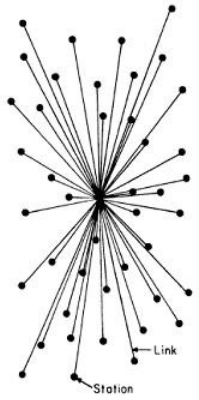
\includegraphics[width=0.4\linewidth]{figures/centralized-network.png}
			\caption{Zentrales soziales Netzwerk}
			\label{fig:central-network}
		\end{subfigure}
		\begin{subfigure}[t]{0.4\linewidth}
			\centering
			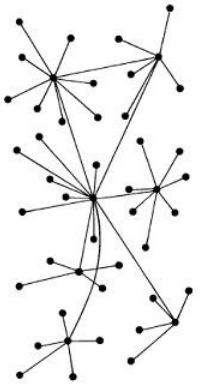
\includegraphics[width=0.4\linewidth]{figures/decentralized-network.png}
			\caption{Dezentrales soziales Netzwerk}
			\label{fig:decentral-network}
		\end{subfigure}
		\vspace{4pt}
		\quelle{(Zentrale, dezentrale, verteilte Systeme \cite{hagengraf})}
		\caption{Klassen sozialer Netzwerke}
	\end{figure}~\\
	In Abbildung 3.2 ist ein zentrales Netzwerk gezeigt welches aus einem zentralen Knoten (Peer) und verschiedenen Blättern (Benutzern) besteht. Fällt der zentrale Knoten aus, können die Nutzer nicht mehr auf das Netzwerk zugreifen was einen großen Flaschenhals aufzeigt.\\
	
	Die Praxis zeigt allerdings, dass ein ausschließlich zentrales System eher selten existiert. Meist sind es Mischformen der verschiedenen Architekturen. Auch große zentrale soziale Netzwerke müssen um Verfügbarkeit u. w. zu gewährleisten verteilte Aspekte haben.\\
	
	Bei einem \textit{dezentralen sozialen Netzwerk} verhält sich das anders. Fällt ein Peer aus, können die Nutzer über andere Instanzen trotzdem weiterhin auf aktive Peers des gesamten Netzwerks zugreifen. Dabei ist allerdings eine erneute Registrierung auf einer weiteren Instanz notwendig. Zudem ist die Kontrolle über Daten auf die einzelnen Peers verteilt anstatt das die gesamten Daten des Netzwerks zentral unter Kontrolle einer Entität stehen. Jedes dezentrale, ist auch ein verteiltes Netzwerk und verfügt somit über eine Middleware Schicht zur Kommunikation der einzelnen Instanzen untereinander.\\
	\todo{Indirektes Professoren Zitat, wie setzt man das um?}
	\begin{figure}[h]
		\begin{minipage}{\textwidth}
			\centering
			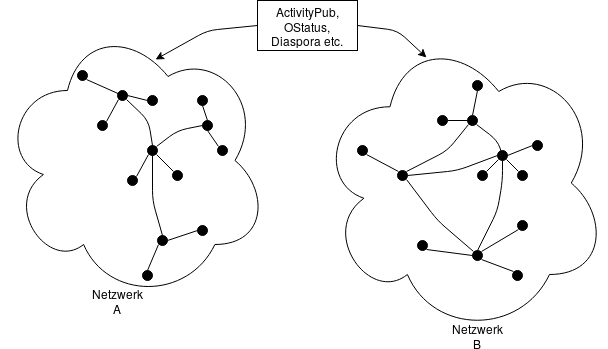
\includegraphics[scale=0.5]{figures/federate.png}
			\label{fig:federated}
			\caption{Förderieren von Netzwerken über verschiedene Protokolle}
		\end{minipage}
	\end{figure}
	Um die Inhalte verschiedener Netzwerke zu verbinden können mehrere soziale Netzwerke zu einem großen verbunden oder \glqq förderiert\grqq~werden. Dies kann über Protokolle und Standards wie OStatus und ActivityPub geschehen oder durch Netzwerkbrücken, im Sinne von Transformatoren, realisiert werden.\\
	
	Da ein dezentrales Netzwerk zugleich auch ein verteiltes ist, betrachten wir folgende allgemeine Definition verteilter Systeme von Andres S. Tanenbaum und Maarten van Steen:
	\begin{addmargin}[1cm]{1cm}
		\vspace{0.5cm}
		\textit{\glqq Ein verteiltes System ist eine Ansammlung unabhängiger Computer, die den Benutzern wie ein einzelnes kohärentes System erscheinen.\grqq}\cite{distributed-systems}
		\vspace{0.5cm}
	\end{addmargin}
	Ein verteiltes Netzwerk ist demnach eine Ansammlung unabhängiger Computer, in diesem Fall die Instanzen eines sozialen Netzwerks, welche den Benutzern wie ein einzelnes kohärentes Netzwerk erscheinen. Die Instanzen können über das \gls{http} Protokoll kommunizieren, was somit die Middleware-Schicht darstellt. Es können Inhalte aus mehreren Instanzen zum Darstellen zusammengetragen werden, was der kohärente Aspekt dabei ist.\\
	
	Das soziale Netzwerk der Firma, für die diese Abschlussarbeit angefertigt wird, hat eine zentrale System Architektur. Die einzelnen Instanzen können also nicht untereinander kommunizieren. Allerdings ist das Netzwerk aus der Sicht her dezentral, als dass jede Person eine eigene Instanz des Netzwerks aufsetzten kann. Zudem ist das Netzwerk bezogen auf die Daten dezentral, da jeder der eine eigene Instanz aufsetzt die Kontrolle über auf dieser generierte Daten hat. Durch die Implementierung des ActivityPub Protokolls wird das System zugleich verteilt und föderiert. Verteilt, weil mit dem Protokoll auch eine Schnittstelle für die Kommunikation der Instanzen des Netzwerks bereitgestellt wird. Förderiert, da diese Schnittstelle auch von anderen Netzwerken implementiert wird und somit die Kommunikation zu Instanzen fremder Netzwerke möglich ist.
	\subsection{
		\iflanguage{english}{Security aspects of social networks}{Sicherheitsaspekte sozialer Netzwerke}
	}
	Es gibt einige Sicherheitsaspekte auf die bei der Entwicklung eines sozialen Netzwerks Wert gelegt werden sollte. Dabei sind einige auch optional, da es denkbar ist, dass ein Netzwerk erstellt wird bei dem z. B. keine Authentisierung notwendig ist. Folgend sind einige Aspekte aufgelistet, auf die geachtet werden sollte:
	\begin{itemize}
		\item Die Authentisierung der Nutzer gegenüber dem Server
		\item Das Sicherstellen der Datenintegrität
		\item Schutz der Datenbank vor unbefugtem Zugriff
		\item Filterung (Nutzer bekommt nur das zu sehen, was er sehen darf)
	\end{itemize}
	Um die einzelnen Nutzer gegenüber dem Server zu authentisieren, können Technologien wie OAuth\footnote{siehe \url{https://tools.ietf.org/html/rfc6749}} oder JSON Web Token\footnote{siehe \url{https://tools.ietf.org/html/rfc7519}} verwendet werden. Dadurch ist sichergestellt, das nur derjenige mit korrekten Anmeldedaten das Profil benutzen kann. Außerdem weiß der Server dadurch wie er die Inhalte Filtern muss um dem Nutzer das für ihn erlaubte anzeigen zu können.\\
	
	Das Sicherstellen der manipulationsfreien Übertragung von Inhalten ist sowohl bei der Client zu Server, als auch bei der Server-zu-Server Kommunikation zu Empfehlen. Bei beiden Kommunikationsszenarien werden die Daten über das Internet übertragen und sind somit potentiell manipulierbar. Sichergestellt werden kann dies z. B. über HTTP-Signaturen s. \ref{subsec:http-signaturen}.\\
	
	Ein weiterer wichtiger Sicherheitsaspekt ist das Schützen der Datenbank vor unbefugtem Zugriff. Bei einem sozialen Netzwerk kann man die Datenbank durchaus als das Herzstück des Netzwerkes bezeichnen, da in dieser, gerade bei \glqq sozialen Netzwerken\grqq~eine riesige Menge an Daten liegen. Schaffen es Angreifer auf diese Zugriff zu bekommen und unbemerkt zu bleiben, kann die Datenbank in Ruhe analysiert oder womöglich die Inhalte auf einen eigenen Server transferiert werden. Durch das isolieren der Datenbank, restriktiven oder keinen direkten Zugriff durch Nutzer oder eine Mehrfaktor Authentisierung kann die Sicherheit der Datenbank erhöht werden.
\section{
	\iflanguage{english}{cryptography}{Kryptographie}
}
	\glqq Unter dem Begriff Kryptographie ist die Wissenschaft vom geheimen Schreiben zu verstehen\grqq~(Vgl. \cite[S. 1]{kryptographie}). Man spricht von symmetrischer Verschlüsselung wenn eine Nachricht im Klartext vom Sender mit einem geheimen Schlüssel, welcher beiden Parteien bekannt ist, verschlüsselt und vom Empfänger, mit demselben Schlüssel, entschlüsselt wird (Vgl. \cite[S. 1]{kryptographie}).
	\begin{figure}[h]
		\begin{minipage}{\textwidth}
			\centering
			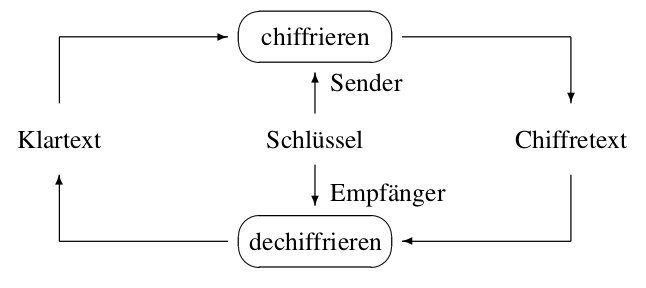
\includegraphics[scale=0.5]{figures/ver-und-entschluesseln.png}
			\quelle{\cite[S. 1]{kryptographie}}
			\label{fig:ver-und-entschluesselung}
			\caption{Symmetrische Ver- und Entschlüsselung}
		\end{minipage}
	\end{figure}
	Von asymmetrischer Verschlüsselung ist die Rede, wenn die Teilnehmer anstatt einen gemeinsamen Schlüssel zu haben, der im vor hinein ausgetauscht werden muss, jeder ein Schlüsselpaar, bestehend aus öffentlichem und privatem Schlüssel, besitzt.\\
	\subsection{RSA}
	Das \gls{rsa} Verfahren ist ein solches asymmetrisches Verschlüsselungsverfahren welches von den drei namens gebenden Mathematikern 1977 entwickelt wurde (Vgl. \cite[S. 77]{kryptographie}). Das \gls{rsa} Verfahren ist wohl das am häufigsten verwendete Public-Key-Kryptosystem.\\
	
	\textbf{Beispiel 1.} Die Gesprächspartner Alice und Bob, welche beide ein Schlüsselpaar besitzen, wollen miteinander kommunizieren. Alice verschlüsselt einen Nachrichtentext mit dem öffentlichen Schlüssel von Bob und sendet die verschlüsselte Nachricht an Bob. Dieser kann seinerseits mit seinem privaten Schlüssel die Nachricht entschlüsseln (Vgl. \cite[S. 73 f.]{kryptographie}).\\
	\subsection{Signaturen}
	Für die Sicherstellung der Authentizität können sogenannte Signaturen verwendet werden. Das oben kurz erläuterte \gls{rsa} Verfahren kann nicht nur zum Ver- und Entschlüsseln von Nachrichten benutzt werden, sondern auch zum signieren. Dabei wird statt des öffentlichen Schlüssels, der private Schlüssel, zusammen mit einer Hashfunktion, benutzt um eine Signatur zu erzeugen. Diese kann dann mit dem öffentlichen Schlüssel des zugehörigen privaten Schlüssels verifiziert werden.\\
	
	\textbf{Beispiel 2.} Bob möchte eine Nachricht an Alice schicken und sichergehen, dass diese auf dem Weg nicht verändert wurde. Er verwendet seinen privaten Schlüssel und wendet diesen auf eine Nachricht an um eine Signatur zu erzeugen. Beides übermittelt er an Alice. Mit dem öffentlichen Schlüssel von Bob kann die fehlerfreie Übertragung der Nachricht verifiziert werden.\\
	
	Unter einer Hashfunktion versteht man eine Einwegfunktion welche auch zur Signierung verwendet werden kann. Bei solch einer Funktion wird ein Eingangswert auf eine kryptische Zeichenfolge abgebildet. Dies wird sehr oft bei Passwörtern verwendet um diese nicht Umkehrbar aufzubewahren.\\
	\subsection{HTTP Signaturen}
	\label{subsec:http-signaturen}
	Eine \textit{HTTP Signatur} wird verwendet um die Authentizität sicherzustellen. Diese wird als Wert einer \glqq Signature\grqq~Kopfzeile eingetragen und besteht aus mehreren Teilen:
	\begin{itemize}
		\item \textit{\textbf{keyId}}="https://example.org/activitypub/users/lea\#main-key"
		\item \textit{\textbf{algorithm}}="rsa-md4"
		\item \textit{\textbf{headers}}="(request-target) date host content-type"
		\item \textit{\textbf{signature}}="DHeEH0Okmtf1ec/lbM1/F5FiLVfQfbWuoFf9t/TzNZiZ7ak"
	\end{itemize}
	Über die \textit{keyId}, was eine Referenz auf einen Schlüssel darstellt, kann der öffentliche Schlüssel angefragt werden. Dies wird beim verifizieren einer Signatur benötigt um die übertragenen Daten auf ihre Authentizität hin zu prüfen.\\
	
	Welcher Hashing-Algorithmus bei der Erstellung verwendet wurde, kann über das \textit{algorithm} Feld der Signatur nachgeschlagen werden. Zudem muss der Algorithmus bei Erstellung in dieses Feld zum Nachschlagen eingetragen werden.\\
	
	Um die eigentliche Signatur zu erzeugen werden die in \textit{headers} angegebenen Kopfzeilen der HTTP Anfrage verwendet. Somit kann eingeschränkt werden welche Metadaten in die Signierung einfließen.\\
	
	Die bei der Signierung mit gegebenem Hashing-Algorithmus und Kopfzeilen erzeugte Signatur wird in das \textit{signature} Feld der HTTP Signatur eingetragen sowie die HTTP Signatur an sich als \glqq Signature\grqq~Kopfzeile der HTTP Anfrage gesetzt (Vgl. \cite{http-signature}).
\section{ActivityPub Standard}
\iflanguage{english}{}{
	Der ActivityPub Standard wurde am 23 Januar 2018 von der \gls{w3c} empfohlen~(Vgl. \cite{activityPub}) und von einer Arbeitsgruppe des \gls{w3c}, der \gls{swwg} (Vgl. \cite{socialWg,pushSocialWeb}), entwickelt. Diese Gruppe war vom 21. Juli 2014 bis zum 13 Februar 2018 aktiv\cite{socialWg} und entwickelte unter anderem ActivityPub, \gls{asc} (Vgl. \cite{activityStreamsCore}) und \gls{asv}(Vgl. \cite{activityStreamsVocabulary}). Die \gls{swwg} war eine Arbeitsgruppe des \gls{w3c} mit dem Ziel neue Protokolle, Vokabulare und \gls{api}'s zu definieren für den Zugriff auf soziale Inhalte der sogenannten \gls{owp} (Vgl. \cite{social-wg-charter}).\\
	
	ActivityPub definiert zwei Protokollschichten, sowie Konzepte, Sammlungen und Interaktionen für dezentrale soziale Netzwerke. Eine Protokollschicht ist das Client-zu-Server Protokoll (Social API), um Clients den Zugriff auf die neusten an sie gesendeten Inhalte zu ermöglichen sowie zum entgegennehmen von Anfragen die vom Client abgesetzt wurden (Vgl. \cite{activityPub}).
	\begin{figure}[h]
		\begin{minipage}{\textwidth}
			\centering
			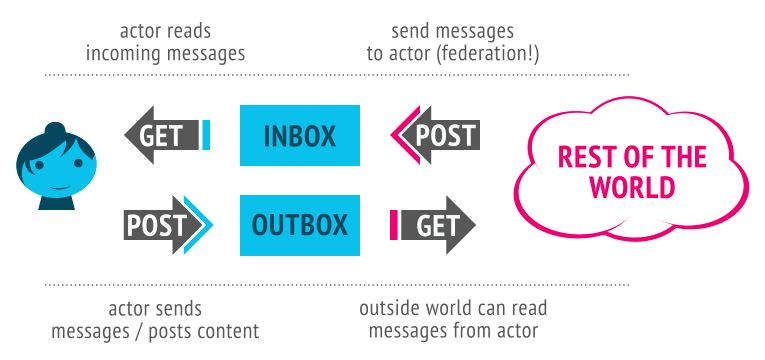
\includegraphics[scale=0.55]{figures/client-server-federated.png}
			\quelle{ActivityPub 2018 - Overview}
			\label{fig:client-server-federated}
			\caption{Schnittstellen des ActivityPub Protokolls}
		\end{minipage}
	\end{figure}
	Die zweite Protokollschicht besteht aus dem förderierten Server-zu-Server Protokoll (Federation Protocol), welches den einzelnen Instanzen von dezentralen sozialen Netzwerken den Austausch von Inhalten untereinander gestattet. ActivityPub setzt auf bereits bestehende Empfehlungen des \gls{w3c} auf, welche teilweise auch von der \gls{swwg} entwickelt wurden wie z. B. \gls{asc} und \gls{asv} (Vgl. \cite{activityPub}). Die zwei Protokollschichten können unabhängig voneinander implementiert werden.\\
	
	Auch andere Technologien wie \gls{JSON-LD} werden verwendet um die Erweiterbarkeit zu gewährleisten. Über neue Ontologien und Vokabulare können weitere syntaktische Definitionen und semantische Beschreibungen zu den bestehenden hinzugefügt werden (Vgl. \cite{activityPub}). Diese Vokabulare können im Kontext des \gls{JSON-LD} Objektes, angegeben werden. Bei ActivityPub wird das \gls{AS2} Vokabular verwendet welches durch \gls{asv} erweitert wird.\\
}
\subsection{
	\iflanguage{english}{Elements of the protocol}{Bestandteile des Protokolls}
}
\iflanguage{english}{}{
	Die Hauptbestandteile des ActivityPub Standards sind die folgenden:
	\begin{itemize}
		\item Aktoren
		\item Objekte
		\item Sammlungen
		\item Aktivitäten
	\end{itemize}
	In ActivityPub werden Benutzer als \glqq Aktoren\grqq(actors) dargestellt (siehe Abb. \ref{fig:actor}). Diese können nicht nur Personen, sondern auch Applikationen, Organisationen, Gruppen und Services sein (Vgl. \cite{activityStreamsCore}). Jedes Aktoren Objekt muss eine \glqq Inbox\grqq~und \glqq Outbox\grqq, welche geordnete Sammlungen sein müssen, sowie einen Identifikator und ein Typ besitzen (Vgl. \cite{activityPub}). Der Identifikator muss global einzigartig sein. Dies kann garantiert werden durch eine Domänen und Protokoll bezogene URI oder IRI wie z. B. \glqq https://example.org/users/alice\grqq~oder \glqq https://example.org/users/álìcê\grqq. Der Typ eines Aktor (z. B. "type": "Person") kann variieren zwischen den fünf oben genannten. Ein Beispiel Aktoren Objekt kann auf der nächsten Seite (Abb. \ref{fig:actor}) begutachtet werden.
	\begin{figure}[h]
		\begin{minipage}{\textwidth}
			\centering
			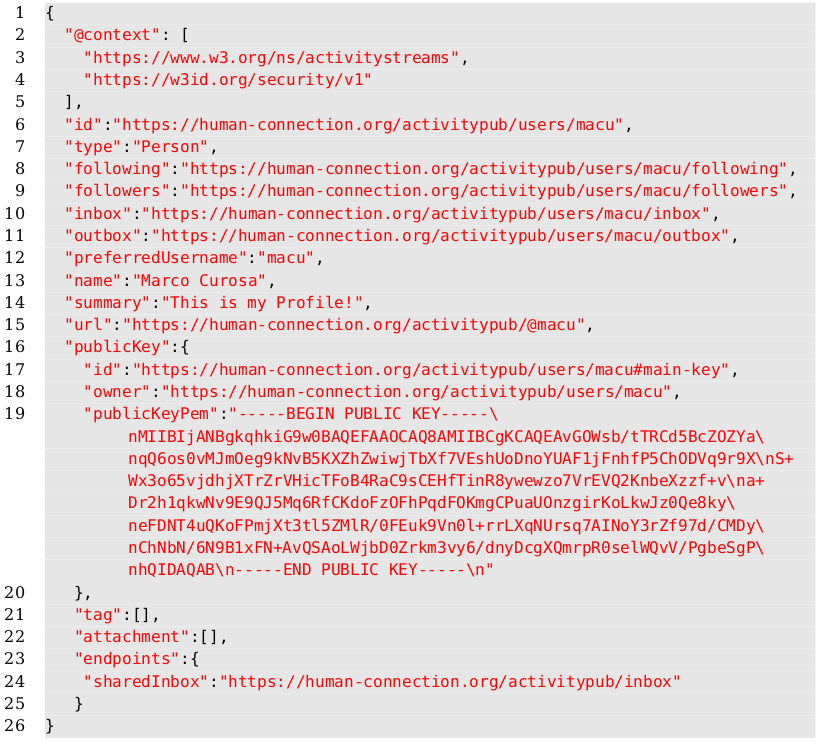
\includegraphics[scale=0.5]{figures/actor.png}
			\label{fig:actor}
			\caption{Beispiel Aktoren Objekt}
		\end{minipage}
	\end{figure}
	Dabei fällt auf das im Kontext des \gls{json-ld} Objektes zwei Einträge zu finden sind. Der erste erweitert das Objekt um die Funktionalität des AS 2.0 Vokabulars und der zweite fügt dem Objekt sicherheitsrelevante Syntax und Semantik hinzu. Der benötigte Identifikator ist hier ein \gls{uri}. Das Aktoren Objekt bildet eine Person mit Namen macu und verschiedenen benötigten sowie optionalen Sammlungen ab. Desweiteren enthält das Objekt eine Beschreibung des Profils (summary) und ein Link zu diesem (url). Aus dem Sicherheitsvokabular wird das \glqq publicKey\grqq~Attribut genutzt. Der Wert ist ein Objekt eines öffentlichen Schlüssels mit einem Identifikator, dem Besitzer und dem eigentlichen Schlüssel im ASCII Format.
}
\subsection{
	\iflanguage{english}{Related standards and components}{Zugehörige Standards und Komponenten}
}
\iflanguage{english}{}{
	Am 22 April 2016 hat die \glqq W3C Community Group\grqq~einen Entwurfsbericht herausgebracht. Durch diesen wird neue Syntax und Semantik definiert um Internet basierten Applikationen das Verschlüsseln, Entschlüsseln sowie digitale Signieren und Verifizieren von verlinkten Daten (Linked Data) zu ermöglichen. Es enthält auch Vokabeln für die Erstellung und Verwaltung einer dezentralen Public-Key-Infrastruktur über das Internet (Vgl. \cite{security-vocab-linked-data}). Ein Anwendungsfall ist das holen des öffentlichen Schlüssels eines Nutzers, über dessen Aktoren Objekt, um eine von Nutzer gesendete Nachricht zu verifizieren.
	\begin{figure}[h]
		\begin{minipage}{\textwidth}
			\centering
			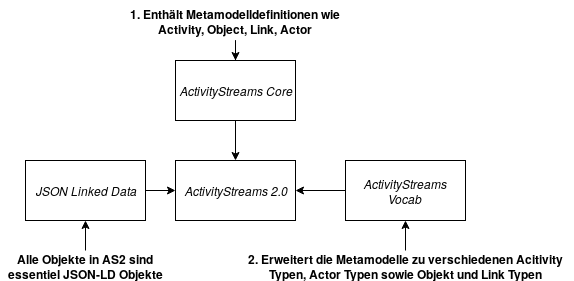
\includegraphics[scale=0.75]{figures/activity-streams.png}
			\label{fig:as2}
			\caption{\gls{as2} Komponenten}
		\end{minipage}
	\end{figure}
	ActivityPub benutzt die \gls{as2} Daten Syntax und das Vokabular. Zusätzlich kann ein weiteres, z. B. das im vorherigen Absatz erwähnte, Sicherheitsvokabular\footnote{Eine Ontologie die Sicherheitsaspekte definiert wie öffentliche Schlüssel, Signaturen u.v.m.} benutzt werden. Auch in Abbildung 3.6 wurde obig beschriebenes Vokabular genutzt.\\
	
	\subsubsection{ActivityStreams 2.0}
	\glqq \gls{as2}\grqq~beinhaltet Modelle für Aktoren, Aktivitäten, Intransitiven Aktivitäten, Objekte, Links, Sammlungen, Natürliche Sprachwerte (Strings) und für Internationalisierung. Das Kernvokabular von \gls{as2} wird durch \gls{asv} erweitert. Dazu gehören verschiedene Aktivitätstypen wie z.B. \glqq Accept\grqq, \glqq Add\grqq, \glqq Remove\grqq, \glqq Delete\grqq~und \glqq Create\grqq, um Aktorentypen wie \glqq Person\grqq, \glqq Application\grqq~und \glqq Group\grqq~sowie um verschiedenste Objekttypen wie \glqq Article\grqq, \glqq Event\grqq, \glqq Note\grqq~und \glqq Relationship\grqq\footnote{siehe \url{https://www.w3.org/TR/activitystreams-vocabulary/}, 3}.\\
	
	Objekte werden innerhalb von \gls{as2} in Aktivitäten eingehüllt um mitteilen zu können das ein Objekt, wie z. B. \glqq Article\grqq, erstellt wurde. Dies geschieht mit der \glqq Create\grqq~Aktivität. Der Mittelpunkt bilden somit Objekte, welche die eigentlichen Inhalte repräsentieren wie Audio oder Video Dateien, Bilder, Artikel und mehr. Die umhüllenden Aktivitäten sind Metadaten um den Objekten erweiterte semantische Informationen zu geben.\\
	
	In den Abbildungen \ref{fig:object-note} und \ref{fig:object-article} sind zwei Beispiel \gls{as2} Objekte abgebildet um die Struktur solcher zu veranschaulichen.\\
	\begin{figure}[h]
		\begin{minipage}{\textwidth}
			\centering
			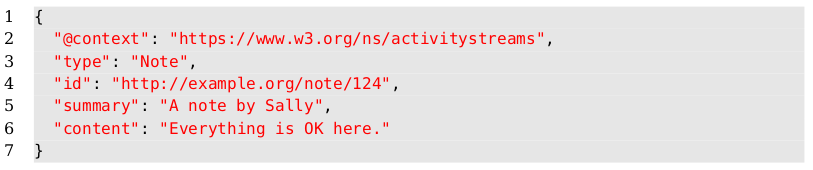
\includegraphics[scale=0.5]{figures/object-note.png}
			\label{fig:object-note}
			\caption{Beispiel Notiz Objekt}
		\end{minipage}
	\end{figure}

	Notizobjekte werden eher für kürzere Texte verwendet. Das prinzipiell wichtigste bei einem Notizobjekt ist der Identifikator sowie der Inhalt. Außerdem kann wie im nachfolgenden Beispiel noch ein veröffentlichungs Attribut, sowie weitere, angegeben werden\footnote{siehe \url{https://www.w3.org/TR/activitystreams-core/}, 4.1}.\\
	\begin{figure}[h]
		\begin{minipage}{\textwidth}
			\centering
			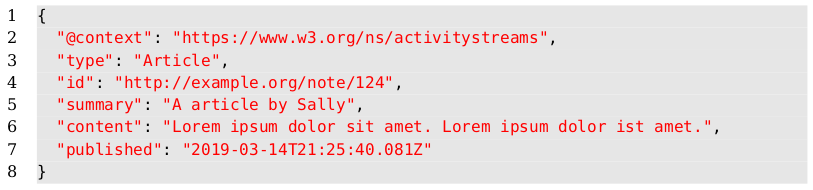
\includegraphics[scale=0.5]{figures/object-article.png}
			\label{fig:object-article}
			\caption{Beispiel Artikel Objekt}
		\end{minipage}
	\end{figure}

	Artikel bilden, im Gegensatz zu Notizen, längere Texte ab. Hier ist, wie oben angedeutet, das Veröffentlichungsdatum mitangegeben.\\
	
	\subsubsection{JSON Linked Data}
	\gls{JSON-LD} ist eine Erweiterung des JSON Formates um verlinkte Daten zu Repräsentieren. JSON an sich, ist ein Format welches im Web häufig Anwendung findet um Daten auszutauschen. Im Kern sind \gls{as2} auch \gls{JSON-LD} Objekte. Der \gls{as2} Kontext definiert verschiedene Klassen und Eigenschaften, von denen nicht alle benutzt werden. Typische Klassen sind \glqq Activity\grqq, \glqq Link\grqq~und \glqq OrderedCollection\grqq.\\
	
	\subsubsection{WebFinger}
	Beim OStatus Protokoll wird zum Entdecken von Profilen für z. B. eine Suchfunktion das WebFinger Protokoll benutzt. Auch dieses Framework verwendet, obwohl der Standard das nicht festlegt, das WebFinger Protokoll. Dabei wird ein \gls{jrd} bereitgestellt, welcher einen Link auf das Aktoren-Objekt enthält. Über diesen kann eine AcitivtyPub konforme Repräsentation eines Nutzern (Aktoren-Objekt) erhalten werden. Beispielsweise wird WebFinger bei Mastodon benutzt um Nutzer zu suchen.
}
\subsection{
	\iflanguage{english}{Authentication and data integrity}{Authentisierung und Datenintegrität}
}
\iflanguage{english}{}{
	Für die Authentisierung und zum sichern der Datenintegrität definiert der Standard keine Mechanismen. Es gibt allerdings \glqq Best Practices\grqq~für die Umsetzung dieser Anforderungen.\\

	Zum einen werden bei der Client-zu-Server Authentisierung \glqq OAuth 2.0 Bearer Tokens\grqq~benutzt, zum anderen, auf der Server Seite, \glqq HTTP\grqq~oder \glqq Linked Data Signatures\grqq~zur Sicherstellung der Datenintegrität.\\
	\label{subsec:authentication:oauth2}
	Bei\glqq OAuth 2.0 Bearer Tokens\grqq~handelt es sich um eine Methode um auf geschützte Ressourcen zugreifen zu können (Vgl. \cite{oauth2}). ActivityPub nutzt diese für jegliche Interaktionen mit dem Server.\\
	
	\glqq Die Datenintegrität umfasst Maßnahmen damit geschützte Daten während der Verarbeitung oder Übertragung nicht durch unautorisierte Personen entfernt oder verändert werden können. Sie stellt die Konsistenz, die Richtigkeit und Vertrauenswürdigkeit der Daten während deren gesamten Lebensdauer sicher und sorgt dafür, dass die relevanten Daten eines Datenstroms rekonstruierbar sind\grqq~(Vgl. \cite{data-integrity}).\\
	
	Um sicherzustellen das HTTP Anfragen beim Transport nicht verändert wurden, können HTTP Signaturen verwendet werden. Diesen verwenden einen kryptografischen Algorithmus um aus ausgewählten Kopfzeilen einer HTTP Anfrage eine kryptischen Zeichenfolge zu generieren. Auf der Empfängerseite kann die Zeichenfolge mit mitgelieferten und auch nachschlagbaren Information verifiziert werden.\\
	
	Wenn ein Objekt nicht nur vom Client zum Server gesendet, sondern auch zwischen Servern untereinander weitergeleitet werden soll wird zum Sicherstellen der Datenintegrität ein anderes Verfahren benötigt als HTTP Signaturen. Die \glqq Best Practices\grqq~empfehlen für solche Fälle \glqq Linked Data Signatures\grqq. Der größte Unterschied zwischen HTTP Signaturen und \glqq Linked Data Signatures\grqq~besteht darin, welche Daten zum Erstellen der Signatur verwendet werden. Bei HTTP Signaturen sind es die Kopfzeilen. Mit \glqq Linked Data Signatures\grqq~kann auch das Objekt selbst, also der Payload einer HTTP Anfrage, anstatt nur die Kopfzeilen, zum signieren verwendet werden.
}
